\chapter{Experimental Setup}

In this chapter, I outline the datasets used in this work, the preprocessing applied to the audio and chord annotations, the evaluation metrics used to compare the models and details of the training process.

\section{Data}

Most of the initial time on this project was spent on finding a suitable dataset for training and testing. \citet{JAAH} use the \emph{JAAH} dataset while \citet{MelodyTranscriptionViaGenerativePreTraining} use the \emph{HookTheory} dataset, defined in Section~\ref{sec:background-data}. Many works use combination of the \emph{McGill Billboard}, \emph{Isophonics}, \emph{RWC-Pop} and \emph{USPop} datasets. However, none have audio freely available. Furthermore, annotations come from different sources in different formats. I spent time looking at scraping audio data, looking at pre-computed features of audio which are available for some datasets and compiling annotations in different formats.

I also spent time contacting authors of previous ACR works to see if they could provide me with audio. I was able to get in contact with Andrea Poltronieri, a PhD student at the University of Bologna and one of the authors of the chord corpus or 'ChoCo' for short~\citep{Choco}. He provided me with labelled audio for the 1217 songs that are commonly used, alongside labelled audio for the \emph{JAAH} dataset. This was a great help despite it coming later in the project than I would have liked.

Therefore, two ACR datasets are used in this work. The first dataset is referred to as the \emph{Pop} dataset as much of the music in the dataset comes from the Billboard Hot 100 charts or other sources of pop music from the last 70 years. This dataset the focus for much of this dissertation. The second dataset is the \emph{JAAH} (Jazz Annotations and Analysis of Harmony) dataset mentioned and is used to assess the generalisation of the model to jazz music. 

The remainder of this section discusses the processing applied to the audio and chord annotations common to both datasets, before discussing details of the \emph{Pop} and \emph{JAAH} datasets relevant to each.

\subsection{Preprocessing}

\subsubsection{Audio to CQT}\label{sec:audio-to-cqt}

The audio was first converted to a Constant-Q Transform (CQT) representation explained in Section~\ref{sec:background-features}. This feature common in ACR and is used as a starting point for this work. The CQT was computed using the \texttt{librosa} library~\citep{librosa}, using the built-in \texttt{cqt} function. A sampling rate of 44100Hz was used, with a hop size of 4096, and 36 bins per octave, 6 octaves and a fundamental frequency corresponding to the note \texttt{C1}. These parameters were chosen to be consistent with previous works~\citep{StructuredTraining} and with common distribution formats. The CQT is returned as a complex-valued matrix containing phase, frequency and amplitude information. Phase information was discarded by taking the absolute value before being converted from amplitude to decibels (dB), equivalent to taking the logarithm.

This leads to a CQT matrix of size $216 \times F$ where 216 is the number of frequency bins and $F$ is the number of frames in the song. The number of frames can be calculated as $F = \lceil \frac{44100}{4096} L  \rceil$ where $L$ is the length of the song in seconds, 44100 is the sampling rate in Hertz (Hz) and 4096 is the hop length in samples. A 3 minute song has just under 2000 frames. To save on computational cost, the CQT was pre-computed into a cached dataset rather than re-computing each CQT on every run.

\subsubsection{Chord Annotations}\label{sec:chord-annotations}

The chord annotation of a song is represented as a sorted dictionary, where each entry contains the chord label, the start time and duration. The chord label is represented as a string in Harte notation~\citep{HarteNotation}. For example, C major 7 is \texttt{C:maj7} and A half diminished 7th in its second inversion is \texttt{A:hdim7/5}. The notation also includes \texttt{N} which signifies that no chord is playing and \texttt{X} symbolising an unknown chord symbol.

This annotation is too flexible to be used as directly as a target for a machine learning classifier trained on limited data. This would lead to thousands of classes, many of which would appear only once. Instead, I define a chord vocabulary. This contains 14 qualities: major, minor, diminished, augmented, minor 6, major 6, minor 7, minor-major 7, major 7, dominant 7, diminished 7, half-diminished 7, suspended 2, and suspended 4. \texttt{N} denotes no chord playing and chords outside the vocabulary are mapped to \texttt{X}, a dedicated unknown symbol. Letting $C$ denote the size of the chord vocabulary, $C=12\cdot14 + 2 = 170$. This vocabulary is consistent with much of the literature~\citep{StructuredTraining,FourTimelyInsights,ACRLargeVocab1}. \citet{ACRLargeVocab1} use a more detailed vocabulary by also including inversions but I decide to remain consistent with previous works. As \citet{StructuredTraining} note, $C=170$ is sufficient for the dataset to exhibit significant imbalance in the chord distribution. Their methodology is easily extensible to larger vocabularies. If performance is not yet satisfactory on $C=170$, it is unlikely that performance will improve with a larger vocabulary.

Both training labels and evaluation labels are converted to this vocabulary. If the evaluation labels were kept in the original Harte notation, the model would be unable to identify them.

A simpler chord vocabulary is also sometimes used. This contains only the major and minor quality for each root and the \texttt{N} and \texttt{X} symbols. For example, \texttt{C:maj7} is mapped to \texttt{C:maj} while \texttt{A:hdim7/5} is mapped to \texttt{X}. For this vocabulary, $C=26$. I did some preliminary tests with this vocabulary but quickly found that model performance was similar over the two vocabularies. Results and analysis can be found in Appendix~\ref{app:small_vs_large_vocabulary}. Additionally, the \texttt{majmin} evaluation metric compares chords over this smaller vocabulary and is mentioned in Section~\ref{sec:evaluation}. The simpler vocabulary is not used in the rest of this work.

The method for converting from Harte notation to a symbol in the chord vocabulary is similar to that used by \citet{StructuredTraining} and is detailed in Appendix~\ref{app:chord_mapping}.

Frames are allocated a chord symbol based on which chord is playing at the middle of the frame. While this may not be a perfect solution, frames are $\approx93$ms long which is shorter than the minimum duration of a chord in the dataset. This guarantees that the chord label for every frame plays for at least half the frame. Furthermore, only $4.4\%$ of frames include a chord transition.

\subsection{Pop Dataset}

The \emph{Pop} dataset consists of songs from the \emph{Mcgill Billboard}, \emph{Isophonics}, \emph{RWC-Pop} and \emph{USPop} datasets mentioned in Section~\ref{sec:background-data}. This collection was originally proposed in work by \citet{FourTimelyInsights} in order to bring together some of the known datasets for chord recognition. The dataset consists of a subset of the above source filtered for duplicates and selected for those with annotations available. In total, there are 1,217 songs. The dataset was provided with obfuscated filenames and audio as \texttt{mp3} files and annotations as \texttt{jams} files~\citep{JAMS}. 

\subsubsection{Data Integrity}\label{sec:data-integrity}

Several possible sources of error in the dataset are investigated below.

\textbf{Duplicates:} Files were renamed using provided metadata identifying them by artist and song title. This was done to identify duplicates in the dataset. There was only one: Blondie's `One Way or Another' which had two different recordings. It was removed from the dataset. Automatic duplicate detection was conducted by embedding each audio using mel-frequency cepstral coefficients (MFCC)~\citep{MFCC}. This function is commonly used to embed audio into low dimensions, and is designed to represent the timbre and shape of a song. This provides a fast and easy way of quantifying similarity. Audio was passed through the \texttt{mfcc} provided in \texttt{librosa} with 20 coefficients. A song's embedding is calculated as the mean MFCC over all frames. Cosine similarities were then calculated for all pairs of tracks. None of the top 50 similarity scores yielded any sign of duplication. I proceed with the assumption that there are no further duplicates in the dataset.

\textbf{Chord-Audio Alignment:} It is pertinent to verify that the chord annotations align with the audio. Badly misaligned annotations could make training impossible.

10 songs were manually investigated for alignment issues. This was done by listening to the audio and comparing it to the annotations directly. It became apparent that precise timings of chord changes are ambiguous. The annotations aired on the side of being slightly early but were all well-timed with detailed chord labellings including inversions and upper extensions.

Automatic analysis of the alignment of the audio and chord annotations was also done using cross-correlation of the derivative of the CQT over time and the chord annotations. Correlations were calculated with a varying time lag. A maximum correlation at a lag of zero would indicate good alignment as the audio changes at the same time as the annotation. The derivative of the CQT in the time dimension was estimated using \texttt{librosa}'s \texttt{librosa.feature.delta} function. The chord annotations were converted to a binary vector, where each element corresponds to a frame in the CQT and is 1 if a chord change occurs at that frame and 0 otherwise. Both the CQT derivatives and binary vectors were normalised by subtracting the mean and dividing by the standard deviation. Finally, cross-correlation was computed using \texttt{numpy}'s \texttt{numpy.correlate} function. A typical cross-correlation for a song is shown in Figure~\ref{fig:cross-correlation}. We can see that the cross-correlation repeats every 20 frames or so. Listening to the song, we can interpret the period of repetition as some fraction of a bar-length likely caused by highly correlated drum transients. 

\begin{figure}[H]
    \centering
    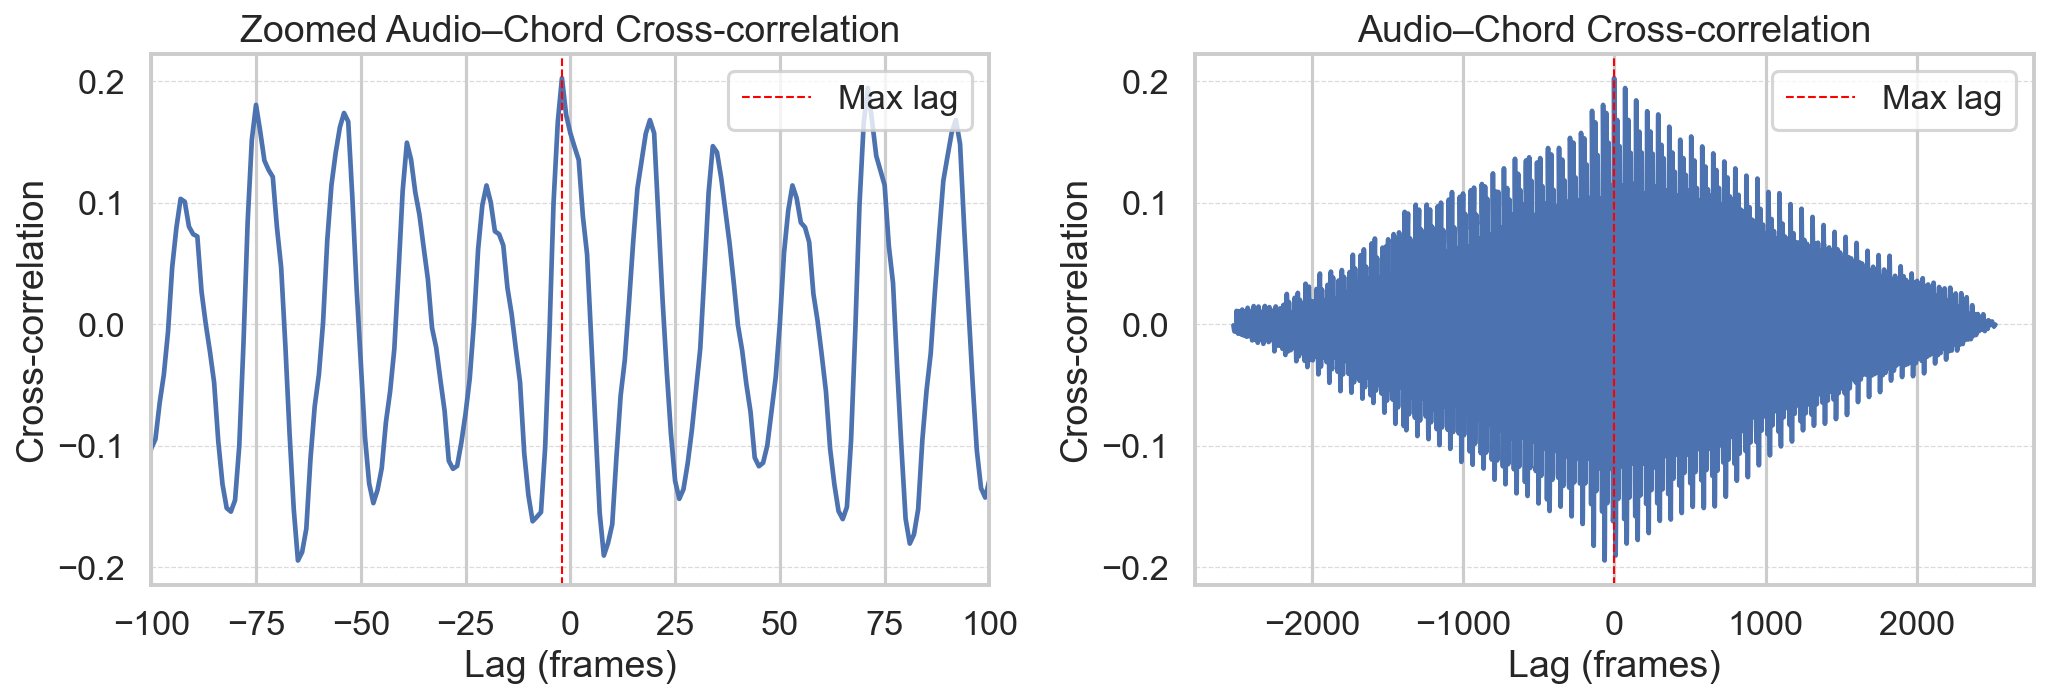
\includegraphics[width=1.0\textwidth]{figures/cross_correlation.png}
    \caption{Cross-correlation of the derivative of the CQT of the audio and the chord annotations for a single song. We can see correlation peaking in regular intervals of around 20 frames. 1 frame is$\approx 0.093$ms so 20 frames $\approx$1.86 seconds. Zooming out, we observe peaks in correlation centred around 0.}\label{fig:cross-correlation}
\end{figure}

To check alignment across the dataset, a histogram of the lag of the maximum cross-correlations over songs is plotted in Figure~\ref{fig:durations-and-lags}. Under the assumption that the annotations are not incorrect by more than 5 seconds, the region of possible maximal lags is restricted to a window of 50 frames either side of 0. This reduction does not change the shape of the picture. Instead, focusing on a reduced set of lags allows more detail to be visible. The majority of songs have a maximum lag close to 0 with a few outliers. This can be attributed to noise. A final check was done by looking at the difference in length of the audio files and chord annotations. A histogram of differences in length is also shown in the figure. The majority of songs have a difference in length of 0, with a few outliers, almost all less than a second. This evidence combined with the qualitative analysis was convincing enough to leave the annotations as they are for training.

\begin{figure}[H]
    \centering
    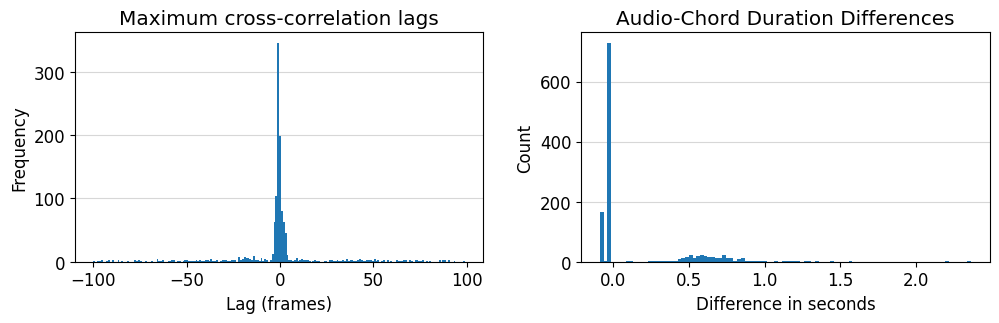
\includegraphics[width=1.0\textwidth]{figures/duration_diffs_and_lags.png}
    \caption{Cross-correlation of the derivative of the CQT of the audio and the chord annotations for a single song. The x-axis is the lag in frames and the y-axis is the correlation. The plot repeats every 100 frames, which corresponds to 4 bars.}\label{fig:durations-and-lags}
\end{figure}

\textbf{Incorrect and Subjective Annotations:} Throughout manual listening, no obviously wrong annotations were found. However, looking at songs which the preliminary models perform the worst on using the \texttt{mirex} metric, three songs stick out. `Lovely Rita' by the Beatles, `Let Me Get to Know You' by Paul Anka and `Nowhere to Run' by Martha Reeves and the Vandellas all had scores below $0.05$. In these songs, the model consistently guessed chords one semitone off, as if it thought the song was in a different key. Upon listening, it became clear that the tuning was not in standard A440Hz for the first two songs and the key of the annotation was wrong for the other. These songs were removed from the dataset. All reported results exclude these data points. No other songs were found to have such issues.

Chord annotations are inherently subjective to some extent. Detailed examples in \emph{Pop} are given by \citet{FourTimelyInsights}. They also note that there are several songs in the dataset of questionable relevance to ACR, as the music itself is not well-explained by chord annotations. However, these are kept in for consistency with other works as this dataset is often used in the literature. Some works decide to use the median as opposed to the mean accuracy in their evaluations in order to counteract the effect of such songs on performance~\citep{StructuredTraining}. We think that this is unnecessary as the effect of these songs is likely to be small and we do not wish to inadvertently inflate our results. Further evidence for use of the mean is given in Section~\ref{sec:evaluation}.

\subsubsection{Chord Distribution}

Much of the recent literature has focused on the long tail of the chord distribution, using a variety of methods to attempt to address the issue. It is first helpful to understand the distribution of chords in the datasets, shown in Figure~\ref{fig:chord-distribution}. The distribution is broken down both by root and quality, using the chord vocabulary with $C=170$. The plots show that the distribution over qualities is highly skewed, with major and minor chords making up the majority of the dataset and qualities like majorminor and diminished 7th chords playing for two to three orders of magnitude fewer seconds. Another display over chord qualities can be found in the work by \citet{ACRLargeVocab1}. The distribution over roots is far less skewed, although there is a preference for chords in keys with roots at C, D and E and fewer in keys with roots at C\# and F\#.

\begin{figure}[H]
    \centering
    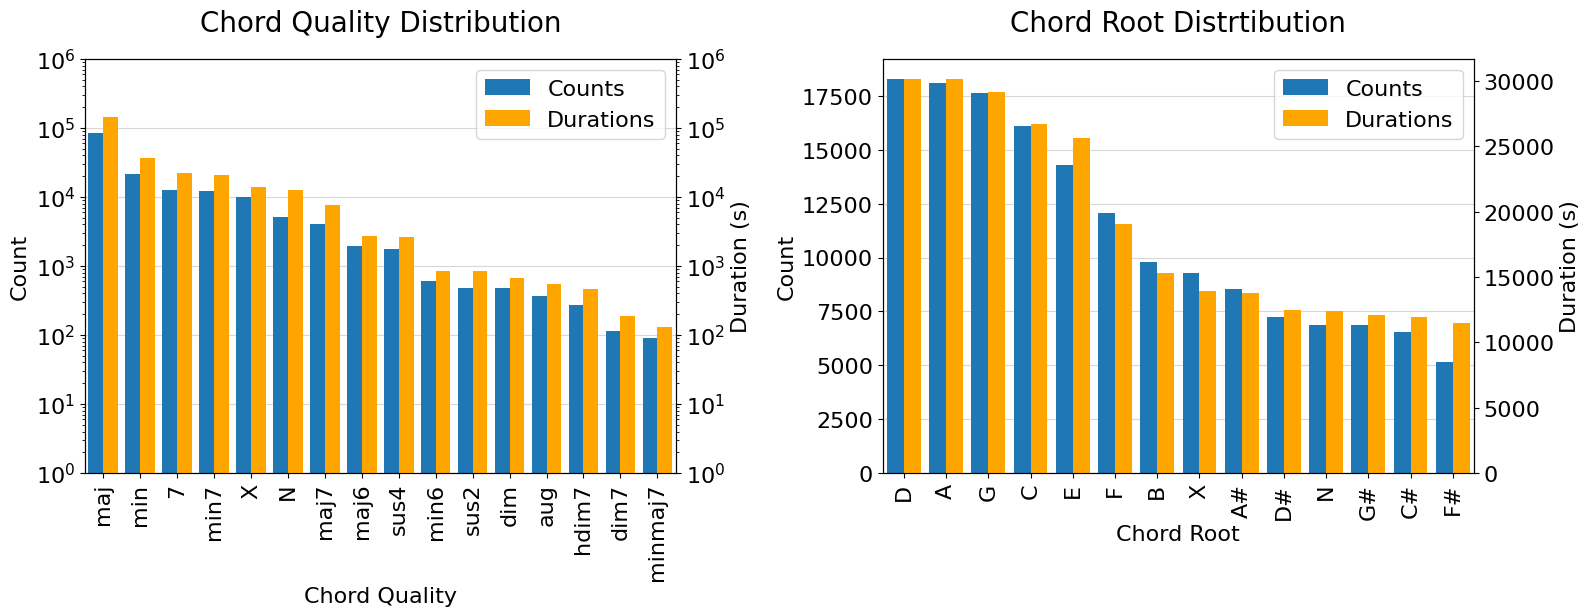
\includegraphics[width=1.0\textwidth]{figures/chord_distribution.png}
    \caption{Chord distributions in the \emph{Pop} dataset. The plots show both the raw counts in terms of frames and the duration in seconds for each chord root/quality. Note that the y-axis over qualities is in a logarithmic scale. We observe that the qualities are very imbalanced, with \texttt{maj} as the most popular. Conversely, roots are relatively balanced.}\label{fig:chord-distribution}
\end{figure}


% \subsection{JAAH Dataset}

% TODO: I was warned by Andrea that the JAAH dataset has not been as commonly used as dataset the Billboard dataset. Therefore he could not guarantee that the audio was aligned for this dataset.

% - As yet, JAAH is unused in this work
% - Data was received as \texttt{.flac} files which were first converted to \texttt{.mp3} files to be in line with the Billboard dataset
% - Comparison of the two datasets
% - Description of the JAAH dataset and its use in this work
% - Intended to be used as a test set to test the synthetic data generation.

\section{Evaluation}\label{sec:evaluation}

As is standard for ACR, weighted chord symbol recall (WCSR) is used to evaluate classifiers. Simply put, WCSR measures the fraction of time that a classifier's prediction is correct. This is defined in Equation~\ref{eq:wcsr}. Correctness can be measured in a variety of ways such as \texttt{root}, \texttt{third} and \texttt{seventh}, which compare the root, root and third, or root, third and seventh respectively. I also make use of the \texttt{mirex} score, where a prediction is correct if it shares at least three notes with the label. This allows for errors like mistaking \texttt{C:7} for \texttt{C:maj} or \texttt{G:maj7} for \texttt{E:min}. Finally, I use \texttt{acc} to denote the overall accuracy where correctness must be exact.

Other measures of correctness are sometimes used. These include \texttt{majmin}, a measure of correctness over only major and minor qualities. I utilise this measure only to substantiate the use of the larger vocabulary in Appendix~\ref{app:small_vs_large_vocabulary}. Measures of correctness over triads and tetrads are also sometimes used, but these are highly correlated with \texttt{third} and \texttt{seventh} respectively. This correlation is to be expected as the third and seventh are strong indicators of the triad and tetrad of the chord. This was also verified empirically on preliminary experiments which are omitted for lack of relevance to the discussion.

These are all implemented in the \texttt{mir\_eval} library~\citep{mir_eval} which also provides utilities for converting discrete Frames-wise chord outputs to intervals from which WCSR can be calculated.

\begin{equation}\label{eq:wcsr}
    WCSR = 100\cdot\frac{1}{Z}\sum_{i=1}^{N} \int_{t=0}^{T_i} M(y_{i,t},\hat{y}_{i,t}) dt
\end{equation}
\begin{equation}
    Z = \sum_{i=1}^{N} \int_{t=0}^{T_i} \mathbb{I}_M(y_{i,t}) dt
\end{equation}

where $M(y, \hat{y})\in\{0,1\}$ is the measure of correctness which varies across metrics. For example, $M(y, \hat{y})$ for \texttt{root} equals $1$ if $y$ and $\hat{y}$ share the same root and $0$ otherwise. $N$ is the number of songs, $T_i$ is the length of song $i$, $y_{i,t}$ is the true chord at time $t$ of song $i$, and $\hat{y}_{i,t}$ is the predicted chord at time $t$ of song $i$. $Z$ normalises by the length of time for which the metric $M$ is defined. This is necessary as \texttt{X} symbols are ignored and \texttt{seventh} ignores some qualities. Further details can be found in the \texttt{mir\_eval} documentation. $\mathbb{I}_M(y_{i,t})=1$ if $M$ is defined for label $y_{i,t}$ and $0$ otherwise. Finally, we multiply by 100 to convert to a percentage.

For the above metrics, the mean is computed over all songs in the evaluation set. Standard errors and 95\% confidence intervals on the means are obtained via bootstrapping. Standard errors are reported for some experiments to provide a sense of the uncertainty in a model's mean performance over songs, not to claim that results are statistically significant.

Some other works report the median. Empirically, I found the median to be $\approx 2\%$ greater than the mean. This may be due to those songs identified as being unsuitable for chordal analysis by \citet{FourTimelyInsights}. I report only the mean throughout this work. This was chosen for being more commonly used in recent literature and because we would to measure the model's performance across songs. It is important for a metric to detect if the model performs poorly over certain genres or styles.

For some experiments, two more metrics are calculated. These are the mean and median class-wise accuracies, called \texttt{acc}\textsubscript{class} and \texttt{median}\textsubscript{class} respectively. \texttt{acc}\textsubscript{class} has previously been defined in terms of discrete frames by \citet{ACRLargeVocab1}. I redefine \texttt{acc}\textsubscript{class} here in terms of WCSR with a similar notation and introduce \texttt{median}\textsubscript{class}. The definitions can be found in Equations~\ref{eq:mean_class_wise} and \ref{eq:mean_class_wise}.

\begin{equation}\label{eq:mean_class_wise}
    \text{acc}\textsubscript{class} = \frac{1}{C} \sum_{c=1}^{C} \text{\emph{WCSR}}(c)
\end{equation}
\begin{equation}\label{eq:median_class_wise}
    \text{median}\textsubscript{class} = \text{median}_{c=1}^{C} [\text{\emph{WCSR}}(c)]
\end{equation}

$C$ denotes the number of chord classes and $\text{\emph{WCSR}}(c)$ is the accuracy of class $c$ is defined in Equation~\ref{eq:wcsr_c}.

\begin{equation}\label{eq:wcsr_c}
    \text{WCSR}(c) = \frac{1}{Z_c}\sum_{i=1}^{N} \int_{t=0}^{T_i} M(y_{i,t},\hat{y}_{i,t}) \cdot \mathbb{I}_c(y_{i,t}) dt
\end{equation}
\begin{equation}
    Z_c = \sum_{i=1}^{N} \int_{t=0}^{T_i} \mathbb{I}_M(y_{i,t})\cdot \mathbb{I}_c(y_{i,t}) dt
\end{equation}

where $N$, $T$, $M$, $y_{i,t}$, $\hat{y}_{i,t}$ and $\mathbb{I}_M(y_{i,t})$ are defined as before in Equation~\ref{eq:wcsr}. $\mathbb{I}_c(y_{i,t})$ is $1$ if the true chord at time $t$ of song $i$ is class $c$ abd $0$ otherwise. $Z_c$ normalises by the length of time for which the chord $c$ is playing and for which the metric $M$ is defined, in a similar fashion to $Z$ in Equation~\ref{eq:wcsr}.

These metrics are intended to measure the model's performance on the long tail of the chord distribution. It is informative to measure both the mean and median to provide a sense of the skew in performance over classes. While the metric can be defined for any measure of correctness, I report only the \texttt{acc} as I found it to be the most informative. For example, the mean class-wise \texttt{root} score is harder to meaningfully interpret.

The justification for redefining \texttt{acc}\textsubscript{class} is that metrics calculated over discrete frames are not comparable across different frame lengths and are dependent on the method for allocating chords to frames. Further, continuous measures more closely reflect what we truly desire from the model. To illustrate this, imagine an extremely large frame length. The model could have perfect scores on these frames be making terrible predictions for most of the song. Through preliminary experiments, it became clear that with sufficiently small hop lengths, there are negligible differences with continuous measures. Nevertheless, there is no reason the field should not adopt a continuous measure of class-wise accuracy.

I do not also compute \emph{quality}-wise accuracies as seen introduced by \citet{CurriculumLearning}. Compared to class-wise metrics, quality-wise metrics only ensure that each root is equally weighted. As roots as fairly balanced, this would not add much information so I do not include it.

For the majority of experiments, the metrics on the validation set are used to compare performance. The test set is held out for use only to compare the final accuracies of selected models in Section~\ref{sec:test-set}.

Finally, other evaluation tools were used such as confusion matrices and the average number of chord transitions per song that a model predicts. Note that confusion matrices were calculated using discrete frames for ease of computation. In an ideal setting, these would also be calculated using continuous measures. I decided it was not worth the additional engineering effort and computational cost given the small differences between the discrete and continuous for sufficiently small frame lengths.

\section{Training}\label{sec:training}

Three variants of the dataset are used for training, validation and testing. For training, an epoch consists of randomly sampling a patch of audio from each song in the training set. The length of this sample is kept as a hyperparameter, set to $10$ seconds for the majority of experiments. For evaluation, the entire song is used because performance was found to be marginally better if the model was allowed to see the entire song at once. This is later discussed in Section~\ref{sec:crnn_performance_across_context}. When validating mid-way through training, songs are split into patches of the same length as the training patches to save on computation time. Samples in a batch are padded to the maximum length of sample in the batch and padded frames are ignored for loss and metric calculation.

Experiments are run on two clusters with some further evaluation taking place locally. The first is The University of Edinburgh's ML Teaching Cluster. Here, NVIDIA GPUs are used - mostly GTX 1080's (10GB VRAM), GTX Titan X's (12GB VRAM) and RTX A6000's (48GB VRAM) depending on the size of experiment and availability on the cluster. Resources have inconsistent availability. Therefore, some experiments are run on The University of Edinburgh's research compute cluster - Eddie. Experiments on Eddie are run on CPUs due to the lack of availability of GPUs. 

Training code is implemented in \texttt{PyTorch}~\citep{pytorch}. Unless stated otherwise, models are trained with the Adam optimiser~\citep{adam} with a learning rate of $0.001$ and pytorch's \texttt{CosineAnnealingLR} scheduler, set to reduce the learning rate to 1/10th of its initial value over the run. Models are trained to minimise the cross entropy loss between the predicted chord and the true chord distribution. I use a batch size of 64 for a maximum of 150 epochs unless stated otherwise. This batch size was found to complete an epoch faster than other batch size tested. Validation part-way through training is conducted every 5 epochs in order to save on computation time. Optionally, training is stopped early if the validation loss does not improve for 25 epochs. The model was is whenever the validation loss improves. Each training run takes approximately 30 minutes of GPU time or 1 hour 30 minutes of CPU time. This can vary up to 10 hours of CPU time for experiments with more expensive computations and larger input. The \texttt{pytorch} seed was set to $0$ for all experiments. 

For the majority of experiments, a random 60/20/20\% training/validation/test split is used. This split is kept constant across experiments. This contrasts much of the literature which uses a 5-fold cross validation introduced by \citet{FourTimelyInsights}. I did not maintain this status quo in order to obtain clean estimators of the generalisation error using the held-out test set and to save on computation time. This makes results hard to compare directly to those reported by the literature. For final testing, models are re-trained on the combined training and validation sets and tested on the test set. To test on the \emph{JAAH} dataset, some models are trained on the entire \emph{Pop} dataset.